\documentclass[12pt]{article}
\usepackage[T2A]{fontenc}
\usepackage[utf8]{inputenc}
\usepackage{multirow}
\usepackage{caption}
\usepackage{subcaption}
\usepackage{amsmath}
\usepackage{changepage}
\usepackage{graphicx}
\usepackage{float}
\usepackage[english,russian]{babel}
\usepackage{amsmath, amsfonts, amssymb, amsthm, mathtools}
\usepackage{xcolor}
\usepackage{array}
\usepackage{hyperref}
\usepackage{icomma}
\usepackage{mathtext} 
\usepackage[top = 1.5cm, left = 1.5 cm, right = 1.5 cm, bottom = 3 cm]{geometry}
\graphicspath{ {./images/} }
 
\title{Колебания в электрических цепях}
\author{Шахматов Андрей, Б02-304}
\date{\today}
  
\begin{document}
\begin{titlepage}
	\begin{center}
		{\large МОСКОВСКИЙ ФИЗИКО-ТЕХНИЧЕСКИЙ ИНСТИТУТ (НАЦИОНАЛЬНЫЙ ИССЛЕДОВАТЕЛЬСКИЙ УНИВЕРСИТЕТ)}
	\end{center}
	\begin{center}
		{\large Физтех-школа физики и исследований им. Ландау}
	\end{center}

	\vspace{3cm}
	{\huge
		\begin{center}
			\textbf{Колебания в электрических цепях}
		\end{center}
	}
	\vspace{2cm}
	\begin{flushright}
		{\LARGE Автор:\\ Шахматов Андрей Юрьевич \\
			\vspace{0.2cm}
			Б02-304}
	\end{flushright}
	\vspace{7 cm}
	\begin{center}
		Долгопрудный 2024
	\end{center}
	\thispagestyle{empty}
\end{titlepage}

% \maketitle

\begin{abstract}

\end{abstract}

% \tableofcontents

\section*{Введение}

\section*{Методика}
\subsection*{Уравнение колебаний в последовательном контуре}
Запишем равенство ЭДС в контуре относительно заряда:
\begin{equation}
	L\ddot{q} + R \dot{q} + \frac{q}{C} = \varepsilon(t),
\end{equation}
где $L$ --- индуктивность катушки, $R$ --- сопротивление резистора, $C$ --- ёмкость контенсатора. 
Поделим на $L$ и введём новые обозначения: 
\[
	\ddot{q} + 2\gamma \dot{q} + \omega_0^2 q = \frac{\varepsilon(t)}{L}, 
\]
где $\gamma = \frac{R}{2L}$ --- коэффициент затухания, $\omega_0 = \sqrt{\frac{1}{LC}}$ --- собственная частота контура. 
Решение такого уравнения представляется в виде суммы частного решения общего решения уравнения: 
\[
	\ddot{q} + 2\gamma \dot{q} + \omega_0^2 q = 0.
\]
Запишем характеристическое уравнение:
\[
	\lambda^2 + 2\gamma \lambda + \omega_0^2 = 0.
\]
Это обыкновенное квадратное уравнение имеет. Запишем его дискриминант: 
\[
	\frac{D}{4} = \gamma^2 - \omega^2
\]
Общее решение имеет вид $\lambda = -\gamma \pm \sqrt{\gamma^2 - \omega^2}$ 
Тогда возможны 3 случая: $\gamma > \omega$, $\gamma = \omega$, $\gamma < \omega$. 
В первом случае дискриминант положителен, во втором случае уравнение имеет два совпадающий решения, 
в третьем случае уравнение имеет два комплексных решения. Можно ввести дополнительную величину
\begin{equation}
	R_{\text{кр}} = 2\sqrt{\frac{L}{C}} > R > 0,  
\end{equation} 
называемая волновым сопротивлением контура.
Тогда общее решение для первого и третьего случая имеет вид: 
\begin{equation}
	q = Ae^{\left( -\gamma + \sqrt{\gamma^2 - \omega^2} \right) t } + Be^{\left( -\gamma - \sqrt{\gamma^2 - \omega^2} \right) t }.  
\end{equation} 
В первом случае уравнение останется в таком виде, тогда заряд будет экспоненциально уменьшаться до нуля, 
колебаний не произойдёт. 
Во третьем случае комплексные экспоненты преобразуются в синусы и косинусы по формуле Эйлера(при этом 
комплексные части сократятся), тогда 
решение можно переписать в виде: 
\begin{equation}
	q = q_0 e^{-\gamma t} \cos(\sqrt{\omega^2 - \gamma^2}t + \varphi_0) = q_0 e^{-\gamma t} \cos(w_1 t + \varphi_0).
\end{equation}
Такой режим представляет затухающие колебания. 
Во втором же случае решение представляет собой 
\begin{equation}
	q = A t e^{\gamma t} + B e^{\gamma t}.
\end{equation}
Такой режим также представляет экспоненциально затухающее апериодическое поведение.
После этого достаточно найти частное решение исходного уравнения и сложить с общим. Аналогичное уравнение может 
быть получено для $U$ на конденсаторе делением полученного уравнения на $C$.  
\subsection*{Установление колебаний}
Рассмотрим внешнее ЭДС изменяющееся по закону:
\[
	\varepsilon = \varepsilon_0 \sin \omega t.
\]
Согласно предыдущему разделу общее решение представляется в виде: 
\[
	U = U_0 e^{-\gamma t} \cos (w_1 t + \varphi_0) + A \cos (wt + \psi).
\] 
Примем в качестве начальных условий $U = 0$, $\dot{U} = 0$ и преобразуем уравнение: 
\[
	U = A \left( \sin (wt + \psi) - e^{-\gamma t} \sin (w_1 t + \psi) \right) 
\]
В случае сильного отличия $w_1$ от $w$ будут наблюдаться биения, однако при небольшом отличие и высокой 
добротности контура уравнение установления колебаний будет иметь вид: 
\begin{equation}
	U = Q \varepsilon_0 \left( 1 - e^{-\gamma t} \right) \sin \omega_0 t,  
\end{equation}  
где $Q$ - добротность контура. 


\subsection*{Описание установки}
\begin{figure}[H]
	\centering
	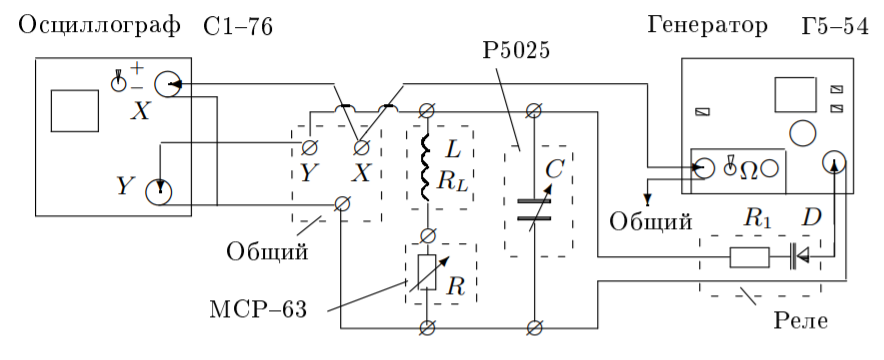
\includegraphics[width=0.6\textwidth]{1.png}
	\caption{Схема установки}
	\label{pic:scheme}
\end{figure}
На рисунке приведена схема для исследования свободных колебаний в контуре, содержащем постоянную индуктивность $L$ и переменные ёмкость $C$ и сопротивление $R$. Колебания наблюдаются на экране осциллографа.

Для периодического возбуждения колебаний в контуре используется генератор импульсов Г5-54. С выхода генератора по коаксиальному кабелю импульсы поступают на колебательный контур через электронное реле, смонтированное в отдельном блоке (или на выходе генератора). Реле содержит тиристор $D$ и ограничительный резистор $R_1$.
Импульсы заряжают конденсатор $C$. После каждого импульса генератор отключается от колебательного контура, и в контуре возникают свободные затухающие колебания. Входное сопротивление осциллографа велико ($\approx 1$ МОм), так что его влиянием на контур можно пренебречь. Для получения устойчивой картины затухающих колебаний используется режим ждущей развёртки с синхронизацией внешними импульсами, поступающими с выхода <<синхроимпульсы>> генератора.

\section*{Результаты и их обсуждение}

\section*{Выводы}
Исследована вольт-амперная характеристика газового разряда. Получены вольт-амперных характеристики 
двойного зонда, помещённого в газовый разряд при различных токах в разряде. Определены основные харастеристики плазмы. 
На основе подученных данных сделан вывод о том, что плазму в газовом разряде можно считать идеальной ($N_D \gg 1$).


\section*{Использованная литература}
\begin{thebibliography}{9}
	\bibitem{LabBook}
	Лабораторный практикум по общей физике, Том 2, под редакцией А. Д. Гладуна
\end{thebibliography}
\end{document}